\documentclass[11pt]{article}
\usepackage[utf8]{inputenc}
\usepackage[ngerman]{babel} % change accordingly

\usepackage{amsmath,amsthm,amssymb,amsfonts}

\usepackage{graphicx}
\graphicspath{{abb/}}
\usepackage{float}
\usepackage{tikz}

\usepackage{fancyhdr} % for headers and footers
\usepackage{geometry}
\usepackage{listings}

\usepackage{hyperref}
\hypersetup{
    linkcolor=blue,     
    urlcolor=cyan,
}

\geometry{
    a4paper, 
    left=20mm,
    right=20mm,
    top=30mm,
    bottom=30mm,
}

\newcommand{\N}{\mathbb{N}}
\newcommand{\Z}{\mathbb{Z}}
\newcommand{\R}{\mathbb{R}}
\newcommand{\Q}{\mathbb{Q}}
\newcommand{\C}{\mathbb{C}}

\newcommand{\e}{\mathrm{e}}

\newcommand{\abs}[1]{\left \lvert #1 \right \rvert}
\newcommand{\floor}[1]{\left \lfloor #1 \right \rfloor}
\newcommand{\ceil}[1]{\left \lceil #1 \right \rceil}

\newcommand{\liminftyn}{\lim\limits_{n \rightarrow \infty}}

\title{Trigonometrie}
\author{Anna Bodnar \& Emil Staikov}
\date{5. März 2021}

\begin{document}
\maketitle
Die trignometrischen Funktionen geben uns die Möglichkeit, verschiedene Größen in Dreiecken zu finden, die wir bis jetzt nicht ohne weiteres ausrechnen konnten. Eine vollständigere mathematische Betrachtung der Trigonometrie werdet ihr im Unterricht noch haben, in diesem Skript werden die grundlegenden Rechenmethoden ohne Beweise dargelegt. \\

\section{Die trigonometrischen Funktionen}
Wir definieren drei grundlegende trignometrische Funktionen mithilfe der Verhältnisse der Seitenlängen in rechtwinkligen Dreiecken, zuerst müssen wir die Seiten jedoch bezeichnen. Ausgehend vom Winkel $\alpha$ nennen wir die gegenüberliegende Seite Gegenkathete (Englisch: opposite) und die kürzere anliegende Seite Ankethete (adjacent). Die im rechtwinkligen Dreieck längste Seite, die auch stets dem rechten Winkel gegenüberliegt (dieser ist auch stets der größte), bezeichnen wir als Hypothenuse (hypothenuse). Wir betrachten das Dreieck immer ausgehend von einem der nicht-rechten Winkel.   
\begin{figure}[ht]
    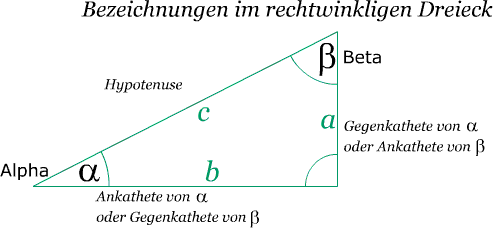
\includegraphics[width=8cm]{seiten-im-rechten-dreieck.png}
    \centering
    \caption{Bezeichnungen im Rechteck}
\end{figure} 
Damit definieren wir nun drei grundlegende Winkelfunktionen: \\
$\displaystyle\sin \alpha = \frac{\text{Gegenkathete}}{\text{Hypothenuse}} \text{ sprich: Sinus}$ \\
$\displaystyle\cos \alpha = \frac{\text{Ankathete}}{\text{Hypothenuse}} \text{ sprich: Kosinus}$ \\
$\displaystyle\tan \alpha = \frac{\sin \alpha}{\cos \alpha} = \frac{\text{Gegenkathete}}{\text{Ankathete}} \text{ sprich: Tangens}$ \\\\
Zum Merken (mithilfe der englischen Bezeichnungen): \\
\textbf{S}ine \textbf{O}pposite \textbf{H}ypothenuse, \textbf{C}osine \textbf{A}djacent \textbf{H}ypothenuse, \textbf{T}angent \textbf{O}pposite \textbf{A}djacent \\
$\implies$ SOHCAHTOA \\\\
Damit können wir in einem Dreieck mit einem bekannten Winkel und einer bekannten Seite die anderen beiden Seiten mit den Winkelfunktionen numerisch bestimmen. Die genauen Werte von $\sin$, $\cos$ und $\tan$ für verschiedene $\alpha$ bleiben erstmal noch ein kleines Mysterium, bald werdet ihr einige besondere Werte aber schon Elementargeometrisch bestimmen können. Im Taschenrechner werden die Werte über sogenannte Taylor-Entwicklungen bestimmt, das werdet ihr aber nicht mal in der Oberstufe zwingend behandeln. In der IJSO solltet ihr immer einen Taschenrechner haben, wenn ihr Werte für trigonometrische Funktionen braucht. \\

Zusätzlich können wir trigonometrische Funktionen umkehren, einem bestimmten Wert können wir stets einen Winkel (uneindeutig) zuordnen. Diese Funktionen heißen $\arcsin$, $\arccos$ und $arctan$ (sprich: Arkus...) und werden auch als $\sin^{-1}$, $\cos^{-1}$ und $\tan^{-1}$ notiert. Sie verhalten sich wie folgt: 
$$\arcsin(\sin(\alpha)) = \arcsin\bigg(\frac{\text{Gegenkathete}}{\text{Hypothenuse}}\bigg) = \alpha$$
Analog verhalten sich $\arccos$ und $\arctan$.

\section{Der Einheitskreis}
Es bietet sich an, den besonderen Fall Hypothenuse mit Länge 1 zu betrachten. Wenn wir den Punkt A (bei Winkel $\alpha$) als Koordinatenursprung wählen, und dann die Gesamtheit aller rechtwinkligen Dreiecke mit Hypothenuse 1 einzeichnen, bilden die Punkte B den sogenannten Einheitskreis, das ist der Kreis um den Ursprung (bzw. A) mit Radius 1 (entspricht jeweils der Hypothenuse). Der Einheitskreis ist in Abb. 2 zu sehen, eingezeichnet sind alle möglichen trignometrischen Funktionen. Im Allgemeinen braucht man aber fast nur $\sin$, $\cos$ und $\tan$. Die Werte für einen Winkel (in der Abbildung $\theta$) sind hier gleich der entsprechenden Längen im Bild, warum dem so ist wird klar, wenn man in die Definitionen für die Hypothenuse 1 einsetzt. Für beliebige rechtwinklige Dreiecke ist das nicht immer der Fall, dort muss man sich die Ausdrücke mit den Definitionen überlegen! \\\\
\begin{figure}[H]
    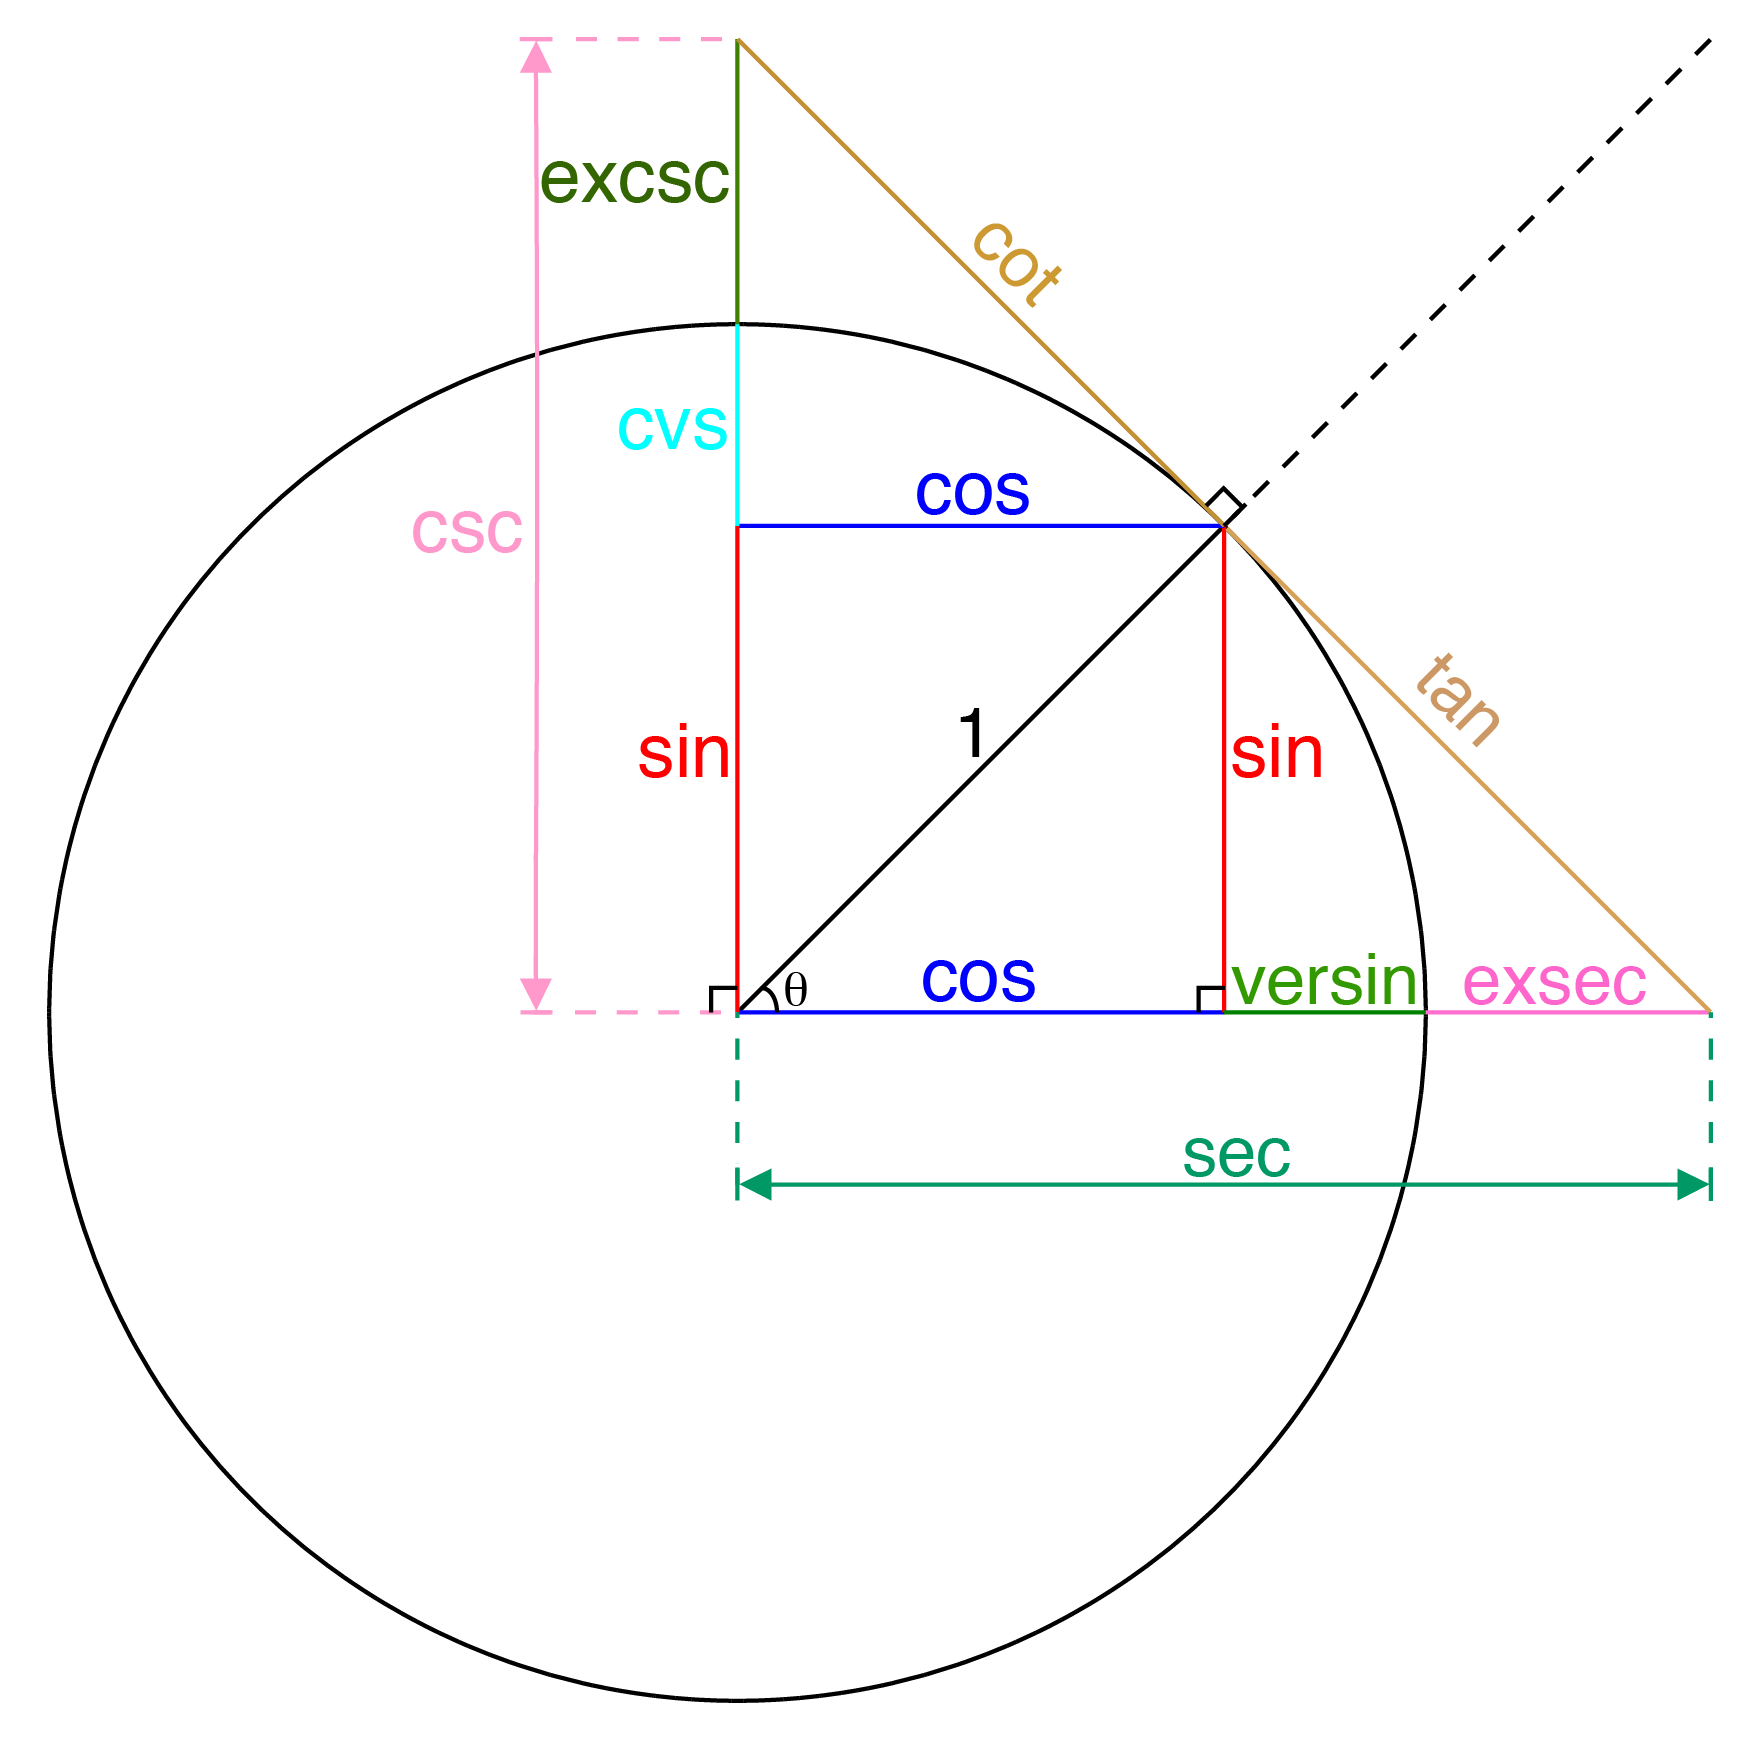
\includegraphics[width=8cm]{einheitskreis-trig-fkt.png}
    \centering
    \caption{Enheitskreis mit trigonometrischen Funktionen}
\end{figure} 
Anhand des Einheitskreises kann man sich mit elementargeometrischen Überlegungen die Werte für $\sin$ (und damit auch direkt $\cos$ und $\tan$, s. Abschnitt 3 bzw. Def. des $\tan$) bestimmter Winkel erschließen. Als Übung: Finde $\sin 30$°, $\sin 45$°, $\sin 60$° \\

Im Einheitskreis bietet es sich an, neben dem schon bekannten Gradmaß (0°, 30°, 60°...) eine neue Winkeleinheit zu definieren, das sogenannte Bogenmaß. Die Größe eines Winkels $\phi$ im Bogenmaß entspricht der Länge, die dieser Winkel auf dem Einheitskreis einschließt (Abb. 3). 
\begin{figure}[ht]
    \includegraphics[width=8cm]{bogenmaß.jpg}
    \centering
    \caption{Bogenmaß}
\end{figure} 
Wir rechnen Grad- und Bogenmaß mit folgendem Sachverhalt ineinander um: 
$$ \frac{\phi}{360} = \frac{b}{2\pi} $$
$b$ ist dabei $\phi$ in Bogenmaß. Diese Umbenennung ist nicht notwendig, man kann auch meistens sowohl mit Bogenmaß als auch mit Gradmaß rechnen, man muss aber konsisten bleiben. Rechnet als Übung einige zufällig gewählte Winkel um. \\
Die absolute einem Winkel entsprechende Bogenlänge in einem Kreis mit einem beliebigen Radius $r$ berechnet sich zu $s = \phi r$, für diese Berechnung muss $\phi$ im Bogenmaß sein.

\section{Sätze in der Trigonometrie}
Mit den Winkelfunktionen ergeben sich verschiedene Sätze, hier ohne Beweis. Mit diesen können wir trigonometrische Gleichungen lösen, aber auch Längen in beliebigen Dreiecken ausrechnen. \\\\
\textbf{Trigonometrischer Pythagoras:} $$1 = \sin^2 x + \cos^2 x$$ wobei $sin^2x = (\sin x)^2$ (Beweis: Satz von Pythagoras im Einheitskreis anwenden). Mit dem trignometrischen Pythagoras können wir Sinus und Kosinus von einem $x$ durcheinander ersetzen. Jetzt kannst du auch $\cos$ und $\tan$ für die im Abschnitt zum Einheitskreis genanneten Winkel ermitteln. \\\\
\textbf{Sinussatz:} In jedem beliebigen Dreieck gilt 
$$\frac{a}{\sin\alpha} = \frac{b}{\sin\beta} = \frac{c}{\sin\gamma}$$ 
\textbf{Kosinussatz:} In jedem beliebigen Dreieck gilt 
$$a^2 = b^2 + c^2 - 2bc \cos \alpha$$ 
$$b^2 = a^2 + c^2 - 2ac \cos \beta$$ 
$$c^2 = a^2 + b^2 - 2bc \cos \gamma$$ 
\textbf{Winkelsummenidentitäten:}
$$\sin{(\alpha \pm \beta)} = \sin\alpha\cos\beta \pm \cos\alpha\sin\beta$$
$$\cos{(\alpha \pm \beta)} = \cos\alpha\cos\beta \mp \sin\alpha\sin\beta$$
Insbesondere kann man daraus auch auf Formeln für $2\theta = \theta + \theta$ schließen. \\\\
\textbf{Symmetrien:} Zeichnet euch die entsprechenden Strecken im Einheitskreis ein. Mit Überlegungen am Einheitskreis kann man sich viele der Identitäten wieder überlegen, sogar wenn man sie mal vergessen hat. Die Identitäten für $\tan$ folgen aus den Ergebnissen für $\sin$ und $\cos$. 
$$\sin(-x) = -\sin x$$
$$\cos(-x) = +\cos x$$
$$\tan(-x) = -\tan x$$
\textbf{Phasenverschiebungen:} Zeichnet euch die entsprechenden Strecken hier erneut im Einheitskreis ein.
$$\sin(x+0.5\pi) = \cos(x)$$ 
$$\cos(x+0.5\pi) = -\sin(x)$$
Es gibt noch viele andere trigonometrische Identitäten, die hiergenannten braucht man jedoch am öftesten. Die meisten Sätze werden sogar bei aller Wahrscheinlichkeit bei der IJSO nicht gebraucht, sie zu kennen ist trotzdem empfehlenswert. 
\end{document}